\documentclass[12pt,a4paper]{article}

% --- Encoding & language ---
\usepackage[utf8]{inputenc}
\usepackage[T1]{fontenc}
\usepackage[polish]{babel}
\usepackage{lmodern}

% --- Math & symbols ---
\usepackage{amsmath,amssymb,amsthm}
\usepackage{mathtools}
\usepackage{bm}

% --- Layout ---
\usepackage[margin=2.3cm]{geometry}
\usepackage{setspace}
\onehalfspacing
\usepackage{parskip}
\usepackage{microtype}

% --- Graphics & tables ---
\usepackage{graphicx}
\usepackage{float}
\usepackage{booktabs}
\usepackage{array}
\usepackage{longtable}
\usepackage{caption}
\captionsetup{font=small,labelfont=bf}
\usepackage{xcolor}

% --- Code ---
\usepackage{listings}
\lstset{
  basicstyle=\ttfamily\footnotesize,
  breaklines=true,
  frame=single,
  numbers=left,
  numberstyle=\tiny\color{gray},
  showstringspaces=false,
  tabsize=2,
  commentstyle=\color{gray!70!black},
  keywordstyle=\color{blue!60!black}\bfseries,
  stringstyle=\color{green!50!black},
  language=Python
}

% --- Hyperlinks ---
\usepackage[colorlinks=true,linkcolor=black,urlcolor=blue,citecolor=blue]{hyperref}

% --- Header / footer ---
\usepackage{fancyhdr}
\setlength{\headheight}{14.5pt}
\addtolength{\topmargin}{-2.5pt}
\pagestyle{fancy}
\fancyhf{}
\fancyhead[L]{\small \textit{Regułowy system ekspertowy --- pacjent geriatryczny}}
\fancyfoot[C]{\thepage}
\renewcommand{\headrulewidth}{0.4pt}

% --- Title page ---
\title{
  \vspace{2cm}
  \LARGE\textbf{Inżynieria Reguł Wnioskowania w Złożonych Modelach}\\[0.6cm]
  \Large Laboratorium 7\\[0.4cm]
  \large \textit{Regułowy system ekspertowy --- pacjent geriatryczny}\\[0.3cm]
  \normalsize Wariant: \textbf{8 — pacjent geriatryczny (wiek $\ge$ 70)}
}
\author{Jakub Jurzak 59099}
\date{07.05.2026}

\begin{document}
\maketitle
\thispagestyle{empty}
\newpage

\tableofcontents
\newpage

\section{Cel zadania}
Implementacja klasycznego i rozmytego systemu ekspertowego rozpoznającego pacjentów geriatrycznych oraz oceniającego ich ryzyko zdrowotne. Dodanie modułu wyjaśnialności (explainable expert system) z analizą wpływu wieku na decyzję.

\section{Opis problemu}
Podstawowy próg wiekowy ($\ge$ 70 lat) nie oddaje stopniowej natury starzenia. Wymagane jest połączenie reguł binarnych z fuzzy logic, aby uzyskać miękką ocenę ryzyka oraz uzasadnić decyzję dla pacjentów na granicy progu.

\section{Opis danych}
Plik \texttt{pacjenci\_demo\_system\_ekspertowy.csv} ($N=30$). Cechy: \texttt{age, bmi, glucose, systolic\_bp, diastolic\_bp}.

\section{Opis metod}
\textbf{Etap 1.} Reguły binarne (\texttt{IF-THEN}) z wagą pewności i agregacją $\max$ po hipotezach.\\\textbf{Etap 2.} Wnioskowanie Mamdaniego: 5 reguł rozmytych, fuzzifikacja (trapezoid/triangle MF), implikacja (\texttt{min}), agregacja (\texttt{max}), defuzyfikacja centroid.\\\textbf{Etap 3.} Wyjaśnienia lokalne (per pacjent: stopnie MF, aktywacje, wkłady reguł) i globalne (średnie aktywacje w kohorcie).

\section{Opis implementacji}
Plik \texttt{lab7/lab7\_solution.py}. Klasy: \texttt{CrispRule}, \texttt{FuzzyRule}. Funkcje MF: \texttt{mu\_age\_elderly}, \texttt{mu\_sbp\_high}, \dots. Implementacja od podstaw, bez scikit-fuzzy, dla pełnej przezroczystości.

\section{Obliczenia}
Reguły klasyczne:

\begin{table}[H]
\centering
\begin{tabular}{lllr}
\toprule
reguła & warunek & wniosek & waga \\
\midrule
R1\_geriatric\_basic & age \$\textbackslash ge\$ 70 & Geriatric patient & 0.95 \\
R2\_geriatric\_hypertension & age \$\textbackslash ge\$ 70 AND SBP \$\textbackslash ge\$ 140 & Geriatric high CV risk & 0.85 \\
R3\_geriatric\_metabolic & age \$\textbackslash ge\$ 70 AND (BMI \$\textbackslash ge\$ 30 OR glucose \$\textbackslash ge\$ 126) & Geriatric metabolic risk & 0.80 \\
R4\_hypertension & SBP \$\textbackslash ge\$ 140 AND DBP \$\textbackslash ge\$ 90 & Hypertension & 0.90 \\
R5\_diabetes & glucose \$\textbackslash ge\$ 126 & Diabetes & 0.85 \\
\bottomrule
\end{tabular}

\caption{Reguły klasyczne.}
\label{tab:crisp}
\end{table}

Reguły rozmyte:

\begin{table}[H]
\centering
\begin{tabular}{ll}
\toprule
reguła & opis \\
\midrule
F1\_elderly & IF age is elderly THEN risk is medium \\
F2\_elderly\_sbp & IF age is elderly AND SBP is high THEN risk is high \\
F3\_elderly\_glucose & IF age is elderly AND glucose is high THEN risk is high \\
F4\_elderly\_bmi & IF age is elderly AND BMI is high THEN risk is high \\
F5\_middle\_age & IF age is middle THEN risk is low \\
\bottomrule
\end{tabular}

\caption{Reguły rozmyte (Mamdani).}
\label{tab:fuzzy}
\end{table}

Wyniki dla wszystkich pacjentów (skrót):

\begin{table}[H]
\centering
\begin{tabular}{lrrr}
\toprule
patient\_id & age & classical\_geriatric & fuzzy\_risk \\
\midrule
P01 & 24 & 0 & 0.00 \\
P02 & 73 & 1 & 70.78 \\
P03 & 65 & 0 & 33.92 \\
P04 & 49 & 0 & 15.58 \\
P05 & 49 & 0 & 15.58 \\
P06 & 79 & 1 & 70.78 \\
P07 & 24 & 0 & 0.00 \\
P08 & 68 & 0 & 63.17 \\
P09 & 32 & 0 & 0.00 \\
P10 & 24 & 0 & 0.00 \\
P11 & 55 & 0 & 15.58 \\
P12 & 88 & 1 & 70.78 \\
P13 & 70 & 1 & 70.78 \\
P14 & 72 & 1 & 70.78 \\
P15 & 69 & 0 & 64.13 \\
P16 & 74 & 1 & 70.78 \\
P17 & 54 & 0 & 15.58 \\
P18 & 27 & 0 & 0.00 \\
P19 & 78 & 1 & 70.78 \\
P20 & 50 & 0 & 15.58 \\
P21 & 54 & 0 & 15.58 \\
P22 & 44 & 0 & 15.96 \\
P23 & 31 & 0 & 0.00 \\
P24 & 84 & 1 & 50.00 \\
P25 & 74 & 1 & 70.78 \\
P26 & 64 & 0 & 50.00 \\
P27 & 46 & 0 & 15.58 \\
P28 & 77 & 1 & 70.78 \\
P29 & 57 & 0 & 27.10 \\
P30 & 49 & 0 & 15.58 \\
\bottomrule
\end{tabular}

\caption{Wnioski klasyczne i rozmyte dla każdego pacjenta.}
\label{tab:all}
\end{table}


\section{Wyniki}
Z $N=30$ pacjentów: liczba klasyfikowanych jako geriatryczni (klasyczne) = \textbf{10}. Średnie ryzyko (fuzzy) w grupie geriatrycznej = \textbf{68.7}, poza nią = \textbf{18.9}.

\textbf{Wyjaśnienie dla pacjenta P02:}

Pacjent ID = P02, age = 73, BMI = 27.8, glukoza = 101, SBP = 148, DBP = 98.

Stopnie przynależności wejść:

 age $\to$ elderly = 1.00, middle = 0.00; SBP $\to$ high = 1.00; glukoza $\to$ high = 0.00; BMI $\to$ high = 0.27.

Aktywacje reguł rozmytych:

 \textbf{F1\_elderly} ($\alpha=1.00$, contrib = 33.4\%): IF age is elderly THEN risk is medium.

 \textbf{F2\_elderly\_sbp} ($\alpha=1.00$, contrib = 50.0\%): IF age is elderly AND SBP is high THEN risk is high.

 \textbf{F3\_elderly\_glucose} ($\alpha=0.00$, contrib = 0.0\%): IF age is elderly AND glucose is high THEN risk is high.

 \textbf{F4\_elderly\_bmi} ($\alpha=0.27$, contrib = 16.6\%): IF age is elderly AND BMI is high THEN risk is high.

 \textbf{F5\_middle\_age} ($\alpha=0.00$, contrib = 0.0\%): IF age is middle THEN risk is low.

Końcowy wskaźnik ryzyka geriatrycznego (defuzzifikacja centroid): \textbf{70.8/100}.

\section{Wykresy}
\begin{figure}[H]
\centering
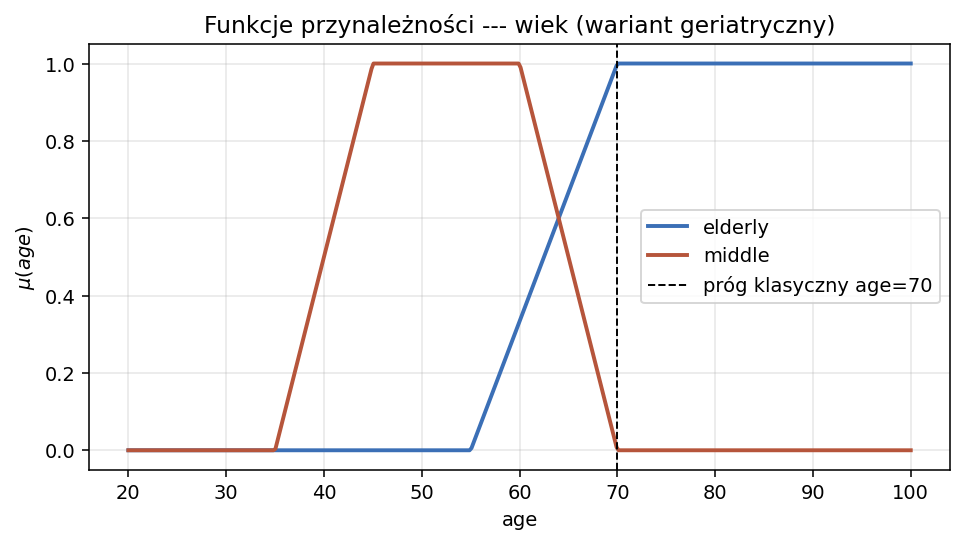
\includegraphics[width=0.85\linewidth]{mf_age.png}
\caption{Funkcje przynależności dla wieku.}
\label{fig:mf-age}
\end{figure}
\begin{figure}[H]
\centering
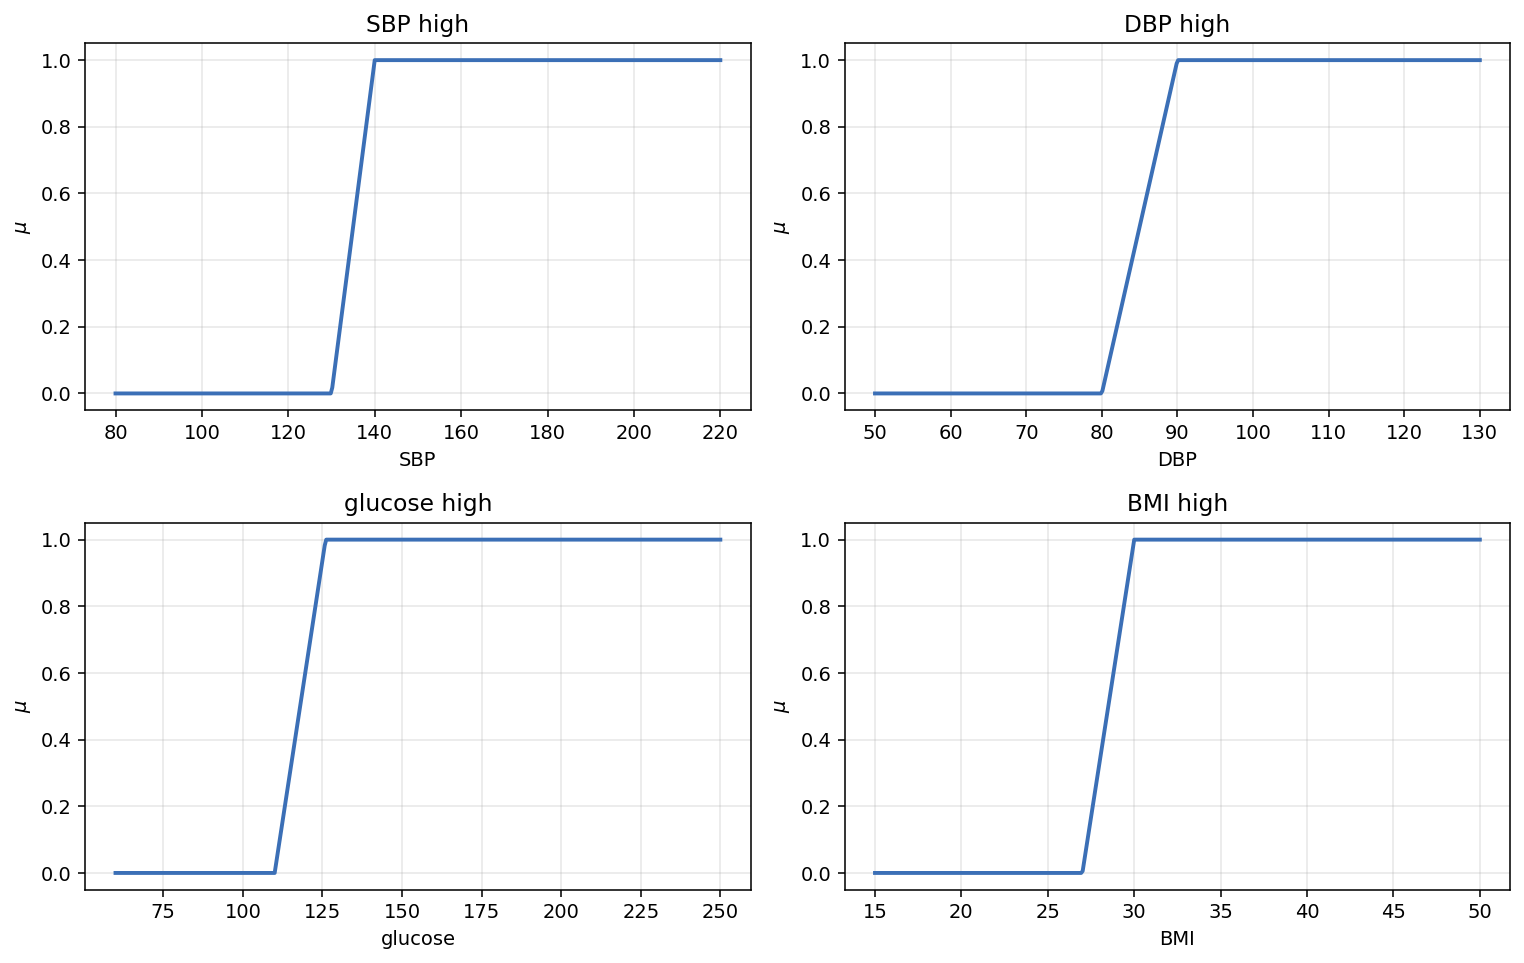
\includegraphics[width=0.85\linewidth]{mf_others.png}
\caption{Pozostałe funkcje przynależności (SBP, DBP, glukoza, BMI).}
\label{fig:mf-rest}
\end{figure}
\begin{figure}[H]
\centering
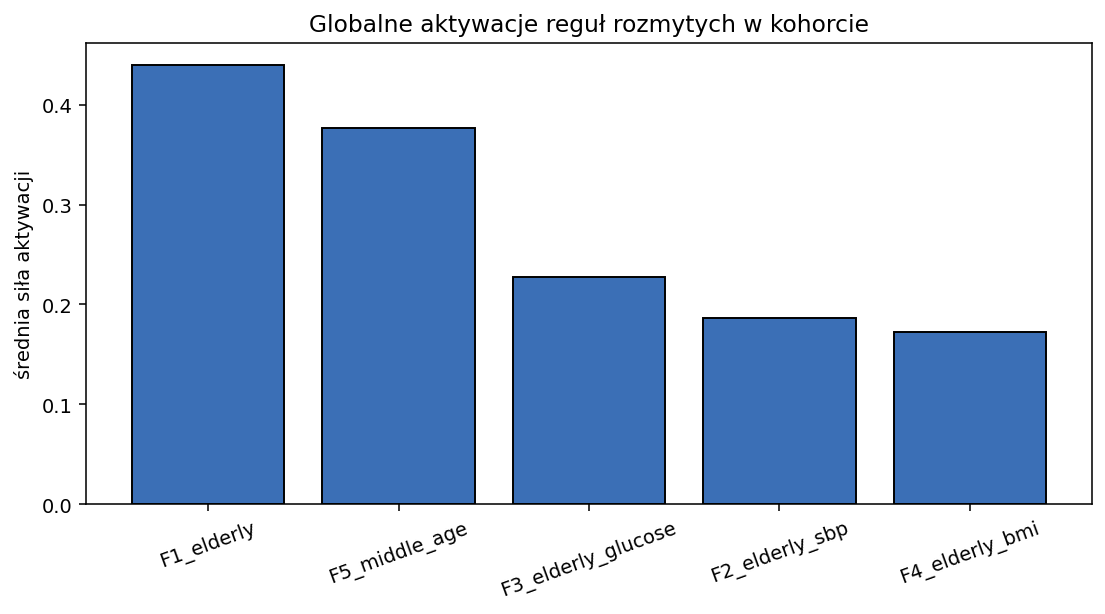
\includegraphics[width=0.85\linewidth]{global_act.png}
\caption{Średnie aktywacje reguł w kohorcie.}
\label{fig:global-act}
\end{figure}
\begin{figure}[H]
\centering
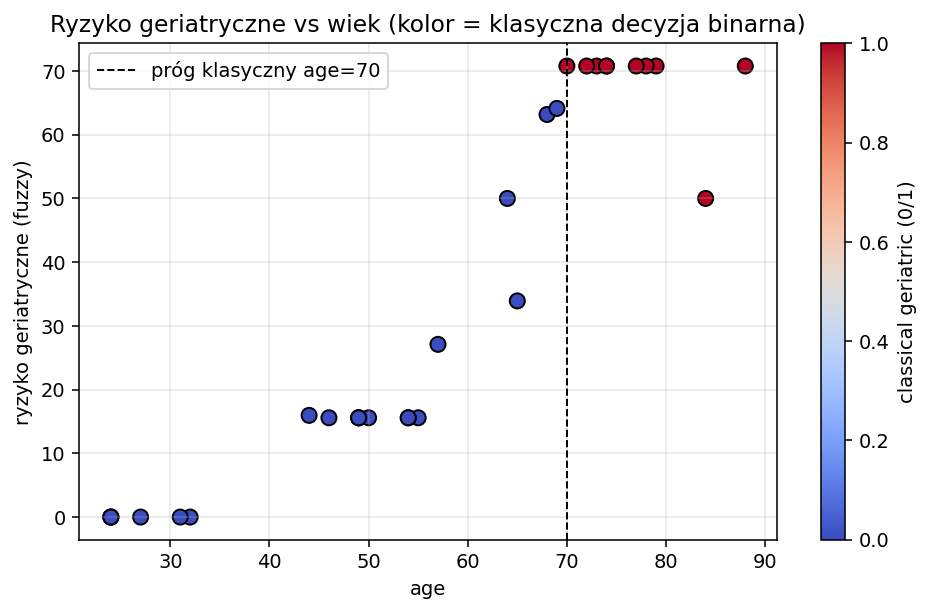
\includegraphics[width=0.85\linewidth]{risk_vs_age.png}
\caption{Ryzyko fuzzy vs wiek z klasyczną decyzją.}
\label{fig:risk-age}
\end{figure}
\begin{figure}[H]
\centering
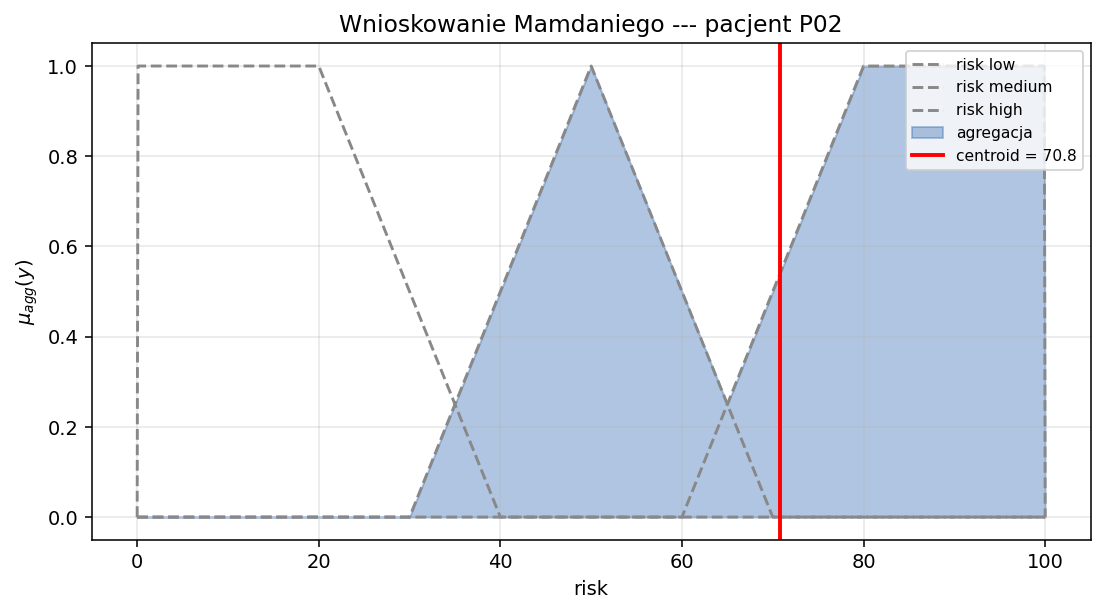
\includegraphics[width=0.85\linewidth]{agg_P02.png}
\caption{Agregacja Mamdaniego --- pacjent P02.}
\label{fig:agg-sample}
\end{figure}


\section{Interpretacja wyników}
Próg wieku $\ge$ 70 jest sztywny: pacjent z wiekiem 69 nie jest klasyfikowany jako geriatryczny w wariancie binarnym, mimo że fuzzy MF \texttt{elderly} aktywuje się częściowo (\texttt{age=69} $\to$ $\mu$ \textgreater 0.9). System rozmyty łagodzi tę nieciągłość. Reguły F2--F4 (geriatric AND komorbidność) zwiększają ryzyko gdy pacjent w podeszłym wieku ma dodatkowe czynniki. Wyjaśnienia lokalne pokazują dokładnie, które reguły i w jakim stopniu zawiodły o końcowej ocenie ryzyka.

\section{Wnioski}
Połączenie reguł klasycznych z rozmytymi pozwala na: (a) zachowanie zgodności z wytycznymi klinicznymi (sztywne progi), (b) realistyczne uchwycenie pacjentów granicznych, (c) interpretowalne wyjaśnienia decyzji. Wkład wieku w końcową ocenę ryzyka jest dominujący dla pacjentów geriatrycznych, ale tylko w połączeniu z innymi czynnikami klinicznymi (SBP, glukoza, BMI). Ograniczenia: brak uczenia się na danych, ręczne kalibrowanie MF, możliwa niespójność reguł.

\end{document}
